\section{Prototype simulations}

\begin{frame}[t]
  \frametitle{Requirements}
  \begin{columns}[T]
    \begin{column}{0.45\textwidth}
      \begin{block}{Requirements on the measurement}
        ESS has specified some requirements:
        \begin{itemize}
          \item Measurement per pulse at nominal conditions
          \item Maximum error on the beam size $<\,10\,\%$
        \end{itemize}
      \end{block}
      \begin{block}{Beam conditions}
        \begin{itemize}
          \item $E_{beam}$: $[97,231,279,316,628]\,\mathrm{MeV}$
          \item Beam $\sigma_{size}$: $[1.8-3]\,\mathrm{mm}$
          \item $i_{beam}=62.5\,\mathrm{mA}$
          \item $t_{pulse}=2.86\,\mathrm{ms}$ ($14\,\mathrm{Hz}$)
        \end{itemize}
      \end{block}
    \end{column}
    \begin{column}{0.45\textwidth}
      \begin{block}{Other requirements}
        \begin{itemize}
          \item Compliant to the use of superconductive cavities nearby
          \item Restricted environnement.
          \item The system must be sustained on a CF200 flange
        \end{itemize}
      \end{block}
      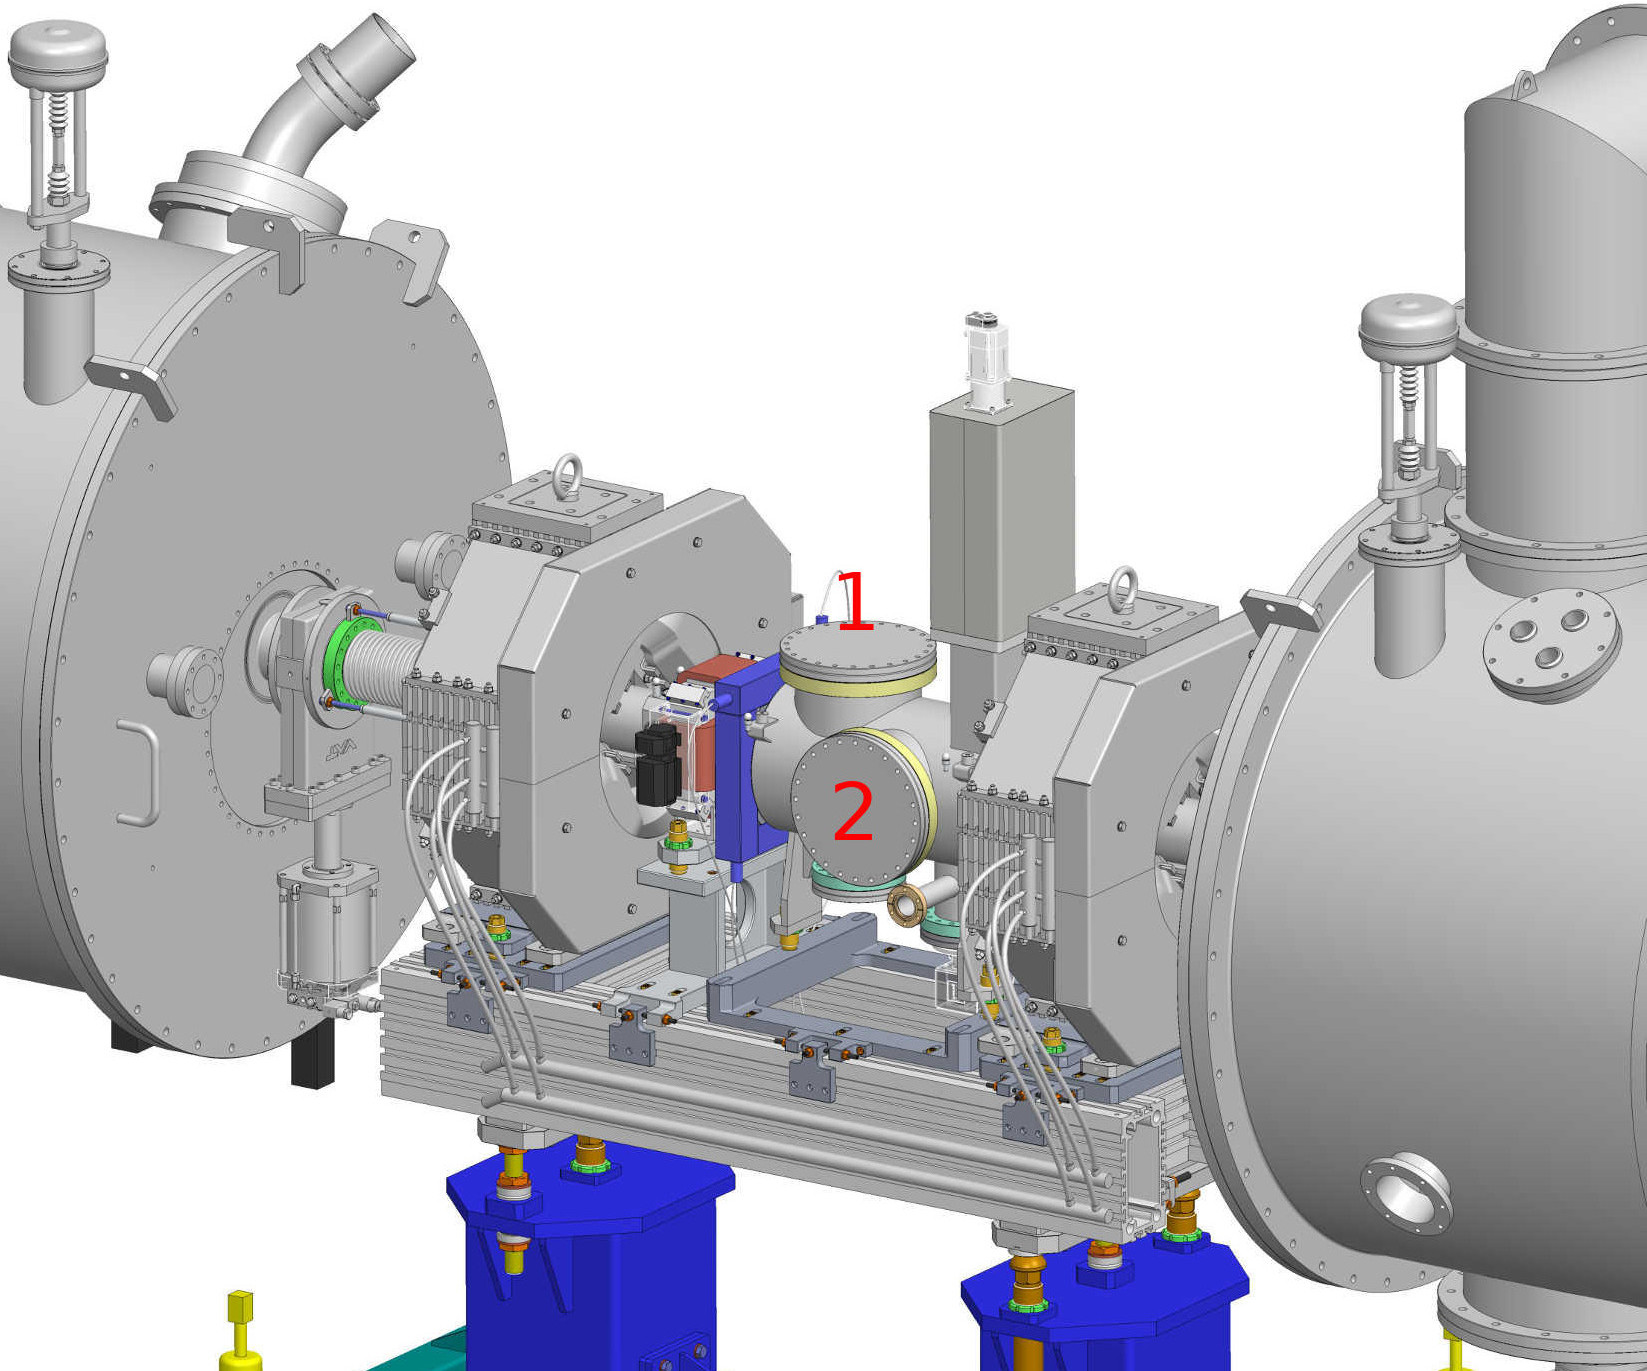
\includegraphics[width=\textwidth]{03_SIM/fig/fig016_LWU_Cryo6}
    \end{column}
  \end{columns}
\end{frame}

\begin{frame}[t]
  \frametitle{IPM}
  \begin{columns}
    \begin{column}{0.45\textwidth}
      \begin{alertblock}{Project is challenging}
        At the beginning of the project, Go/NoGo gate $\implies$ to prove the feasibility.
      \end{alertblock}
      \begin{block}{Each step must be simulated}
        \begin{enumerate}
          \item Quantification of the "primary" ionization signal.
          \item Determination of the $e^-$/ion trajectories during the drift.
          \item The choice of an efficient readout technology.
        \end{enumerate}
      \end{block}
      Each step required different methods and tools
    \end{column}
    \begin{column}{0.45\textwidth}
      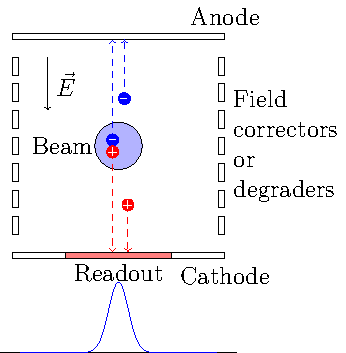
\includegraphics[width=\textwidth]{02_ESS/fig/fig000_IPM.pdf}
    \end{column}
  \end{columns}
\end{frame}

\subsection{Primary ionization signal}
\begin{frame}[t]
  \frametitle{Primary ionization signal}
  \begin{block}{Enough particles to reconstruct a profile?}
    $Signal_{primary} \propto N_{beam}(I_{beam},t_{pulse}) \times \sigma_{ioniz.}(E_{beam},medium)\times \rho$
  \end{block}
  \begin{columns}
    \begin{column}{0.35\textwidth}
      \begin{block}{Conditions}
        \begin{itemize}
          \item Beam:
                \begin{itemize}
                  \item $90\,\mathrm{MeV}$ to $2\,\mathrm{GeV}$
                  \item $62.5\,\mathrm{mA}$
                  \item $2.86\,\mathrm{ms}$
                \end{itemize}
          \item Vacuum: $10^{-9}\,\mathrm{mbar}$
          \item Gas composition:
                \begin{itemize}
                  \item $H_2$ $79\,\%$
                  \item $CO$ $10\,\%$
                  \item $CO_2$ $10\,\%$
                  \item $N_2$ $1\,\%$
                \end{itemize}
        \end{itemize}
      \end{block}
    \end{column}
    \begin{column}{0.60\textwidth}
      \centering
      Bethe stopping power
      \includegraphics[width=\textwidth]{03_SIM/fig/fig000_Bethe_ESS}
    \end{column}
  \end{columns}
\end{frame}

\begin{frame}[t]
  \frametitle{Primary ionization signal}
  \begin{columns}
    \begin{column}{0.55\textwidth}
      \begin{block}{Calculation}
        Two methods:
        \begin{itemize}
          \item Direct calculation with Bethe formula:
                \begin{itemize}
                  \item Straightforward.
                  \item Some parameters are not suitable for vacuum.
                \end{itemize}
          \item Using Garfield++/Heed++ software:
                \begin{itemize}
                  \item Photo Absorption Ionization model
                  \item Take into account the density
                \end{itemize}
        \end{itemize}
      \end{block}
    \end{column}
    \begin{column}{0.35\textwidth}
      \begin{tabularx}{\linewidth}{XX}
        \toprule
        Energy ($\mathrm{MeV}$) & \(N_{garfield}\) per $\mathrm{pulse}/\mathrm{cm}$ \\
        \midrule
        \(97.2\)                & \(52537\)                                         \\
        \(231.4\)               & \(27463\)                                         \\
        \(278.9\)               & \(26124\)                                         \\
        \(315.8\)               & \(23769\)                                         \\
        \(628.3\)               & \(17522\)                                         \\
        \bottomrule
      \end{tabularx}
    \end{column}
  \end{columns}
  \begin{block}{Conclusion}
    Enough particles to reconstruct profile but sensitive readout is mandatory
  \end{block}
  \begin{alertblock}{Limitation}
    Huge dependance on vacuum parameters. Computation only gives an order of magnitude!
  \end{alertblock}
\end{frame}

\subsection{Profile distortions}
\begin{frame}[t]
  \frametitle{Profile distortions}
  \begin{columns}
    \begin{column}{0.45\textwidth}
      A profile measured by an IPM is affected by some distortions
      \begin{block}{Static distortions}
        \begin{itemize}
          \item Do not depend beam/particle status
          \item Can be somehow corrected.
        \end{itemize}
      \end{block}
      \begin{block}{Dynamic distortions}
        \begin{itemize}
          \item Depends on beam/particles status
          \item Hard to correct
          \item Various sources:
                \begin{itemize}
                  \item Space charge
                  \item Initial momentum
                \end{itemize}
        \end{itemize}
      \end{block}
    \end{column}
    \begin{column}{0.45\textwidth}
      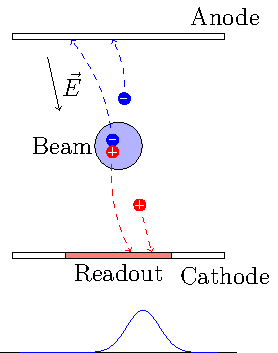
\includegraphics[width=\textwidth]{03_SIM/fig/fig000_IPM_distorsion.pdf}
    \end{column}
  \end{columns}
\end{frame}

\begin{frame}[t]
  \frametitle{Field uniformity}
  \begin{columns}[T]
    \begin{column}{0.45\textwidth}
      \begin{block}{Extraction field is not perfect}
        The non uniformities come from:
        \begin{itemize}
          \item IPM geometry itself, side effects.
          \item The vacuum vessel that encloses the IPM.
          \item IPM polarization.
          \item Other elements in vacuum.
        \end{itemize}
        The uniformity can be improved by hardware corrections.
      \end{block}
    \end{column}
    \begin{column}{0.45\textwidth}
      Example from simulations:
      \begin{center}
        \only<1->{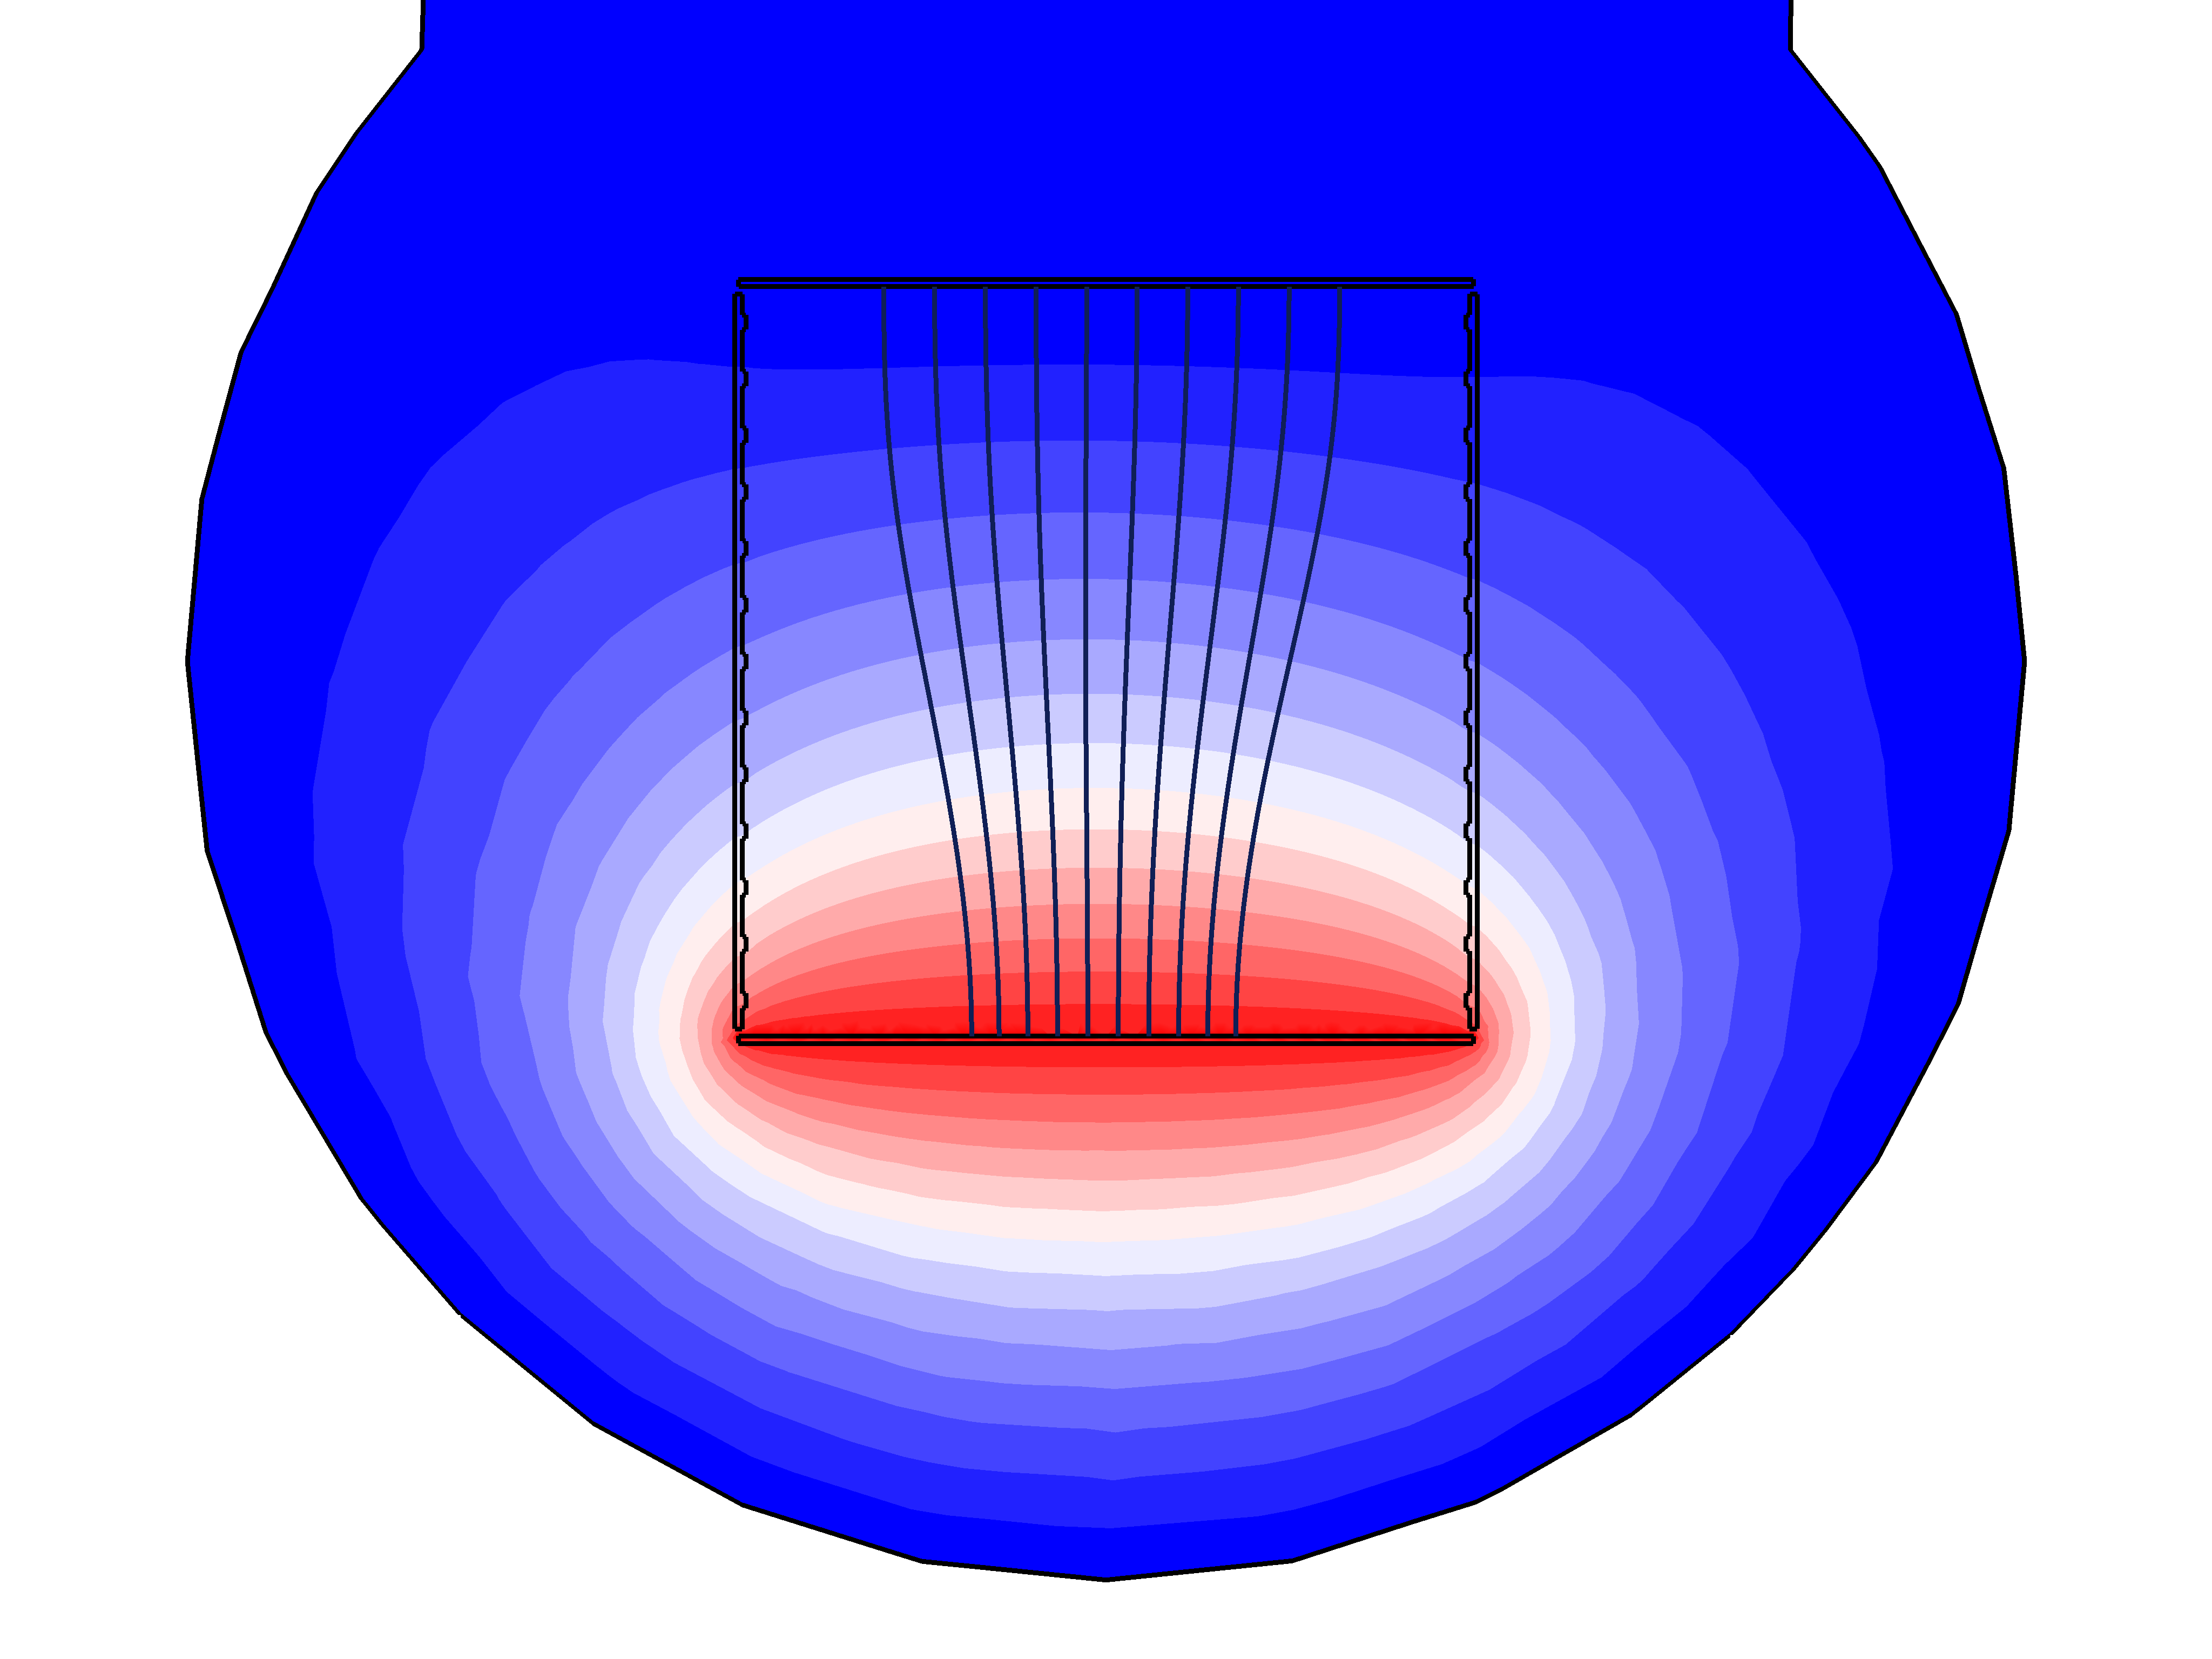
\includegraphics[width=0.9\textwidth]{03_SIM/fig/fig000_Lines_Nocorr}}
        \only<2>{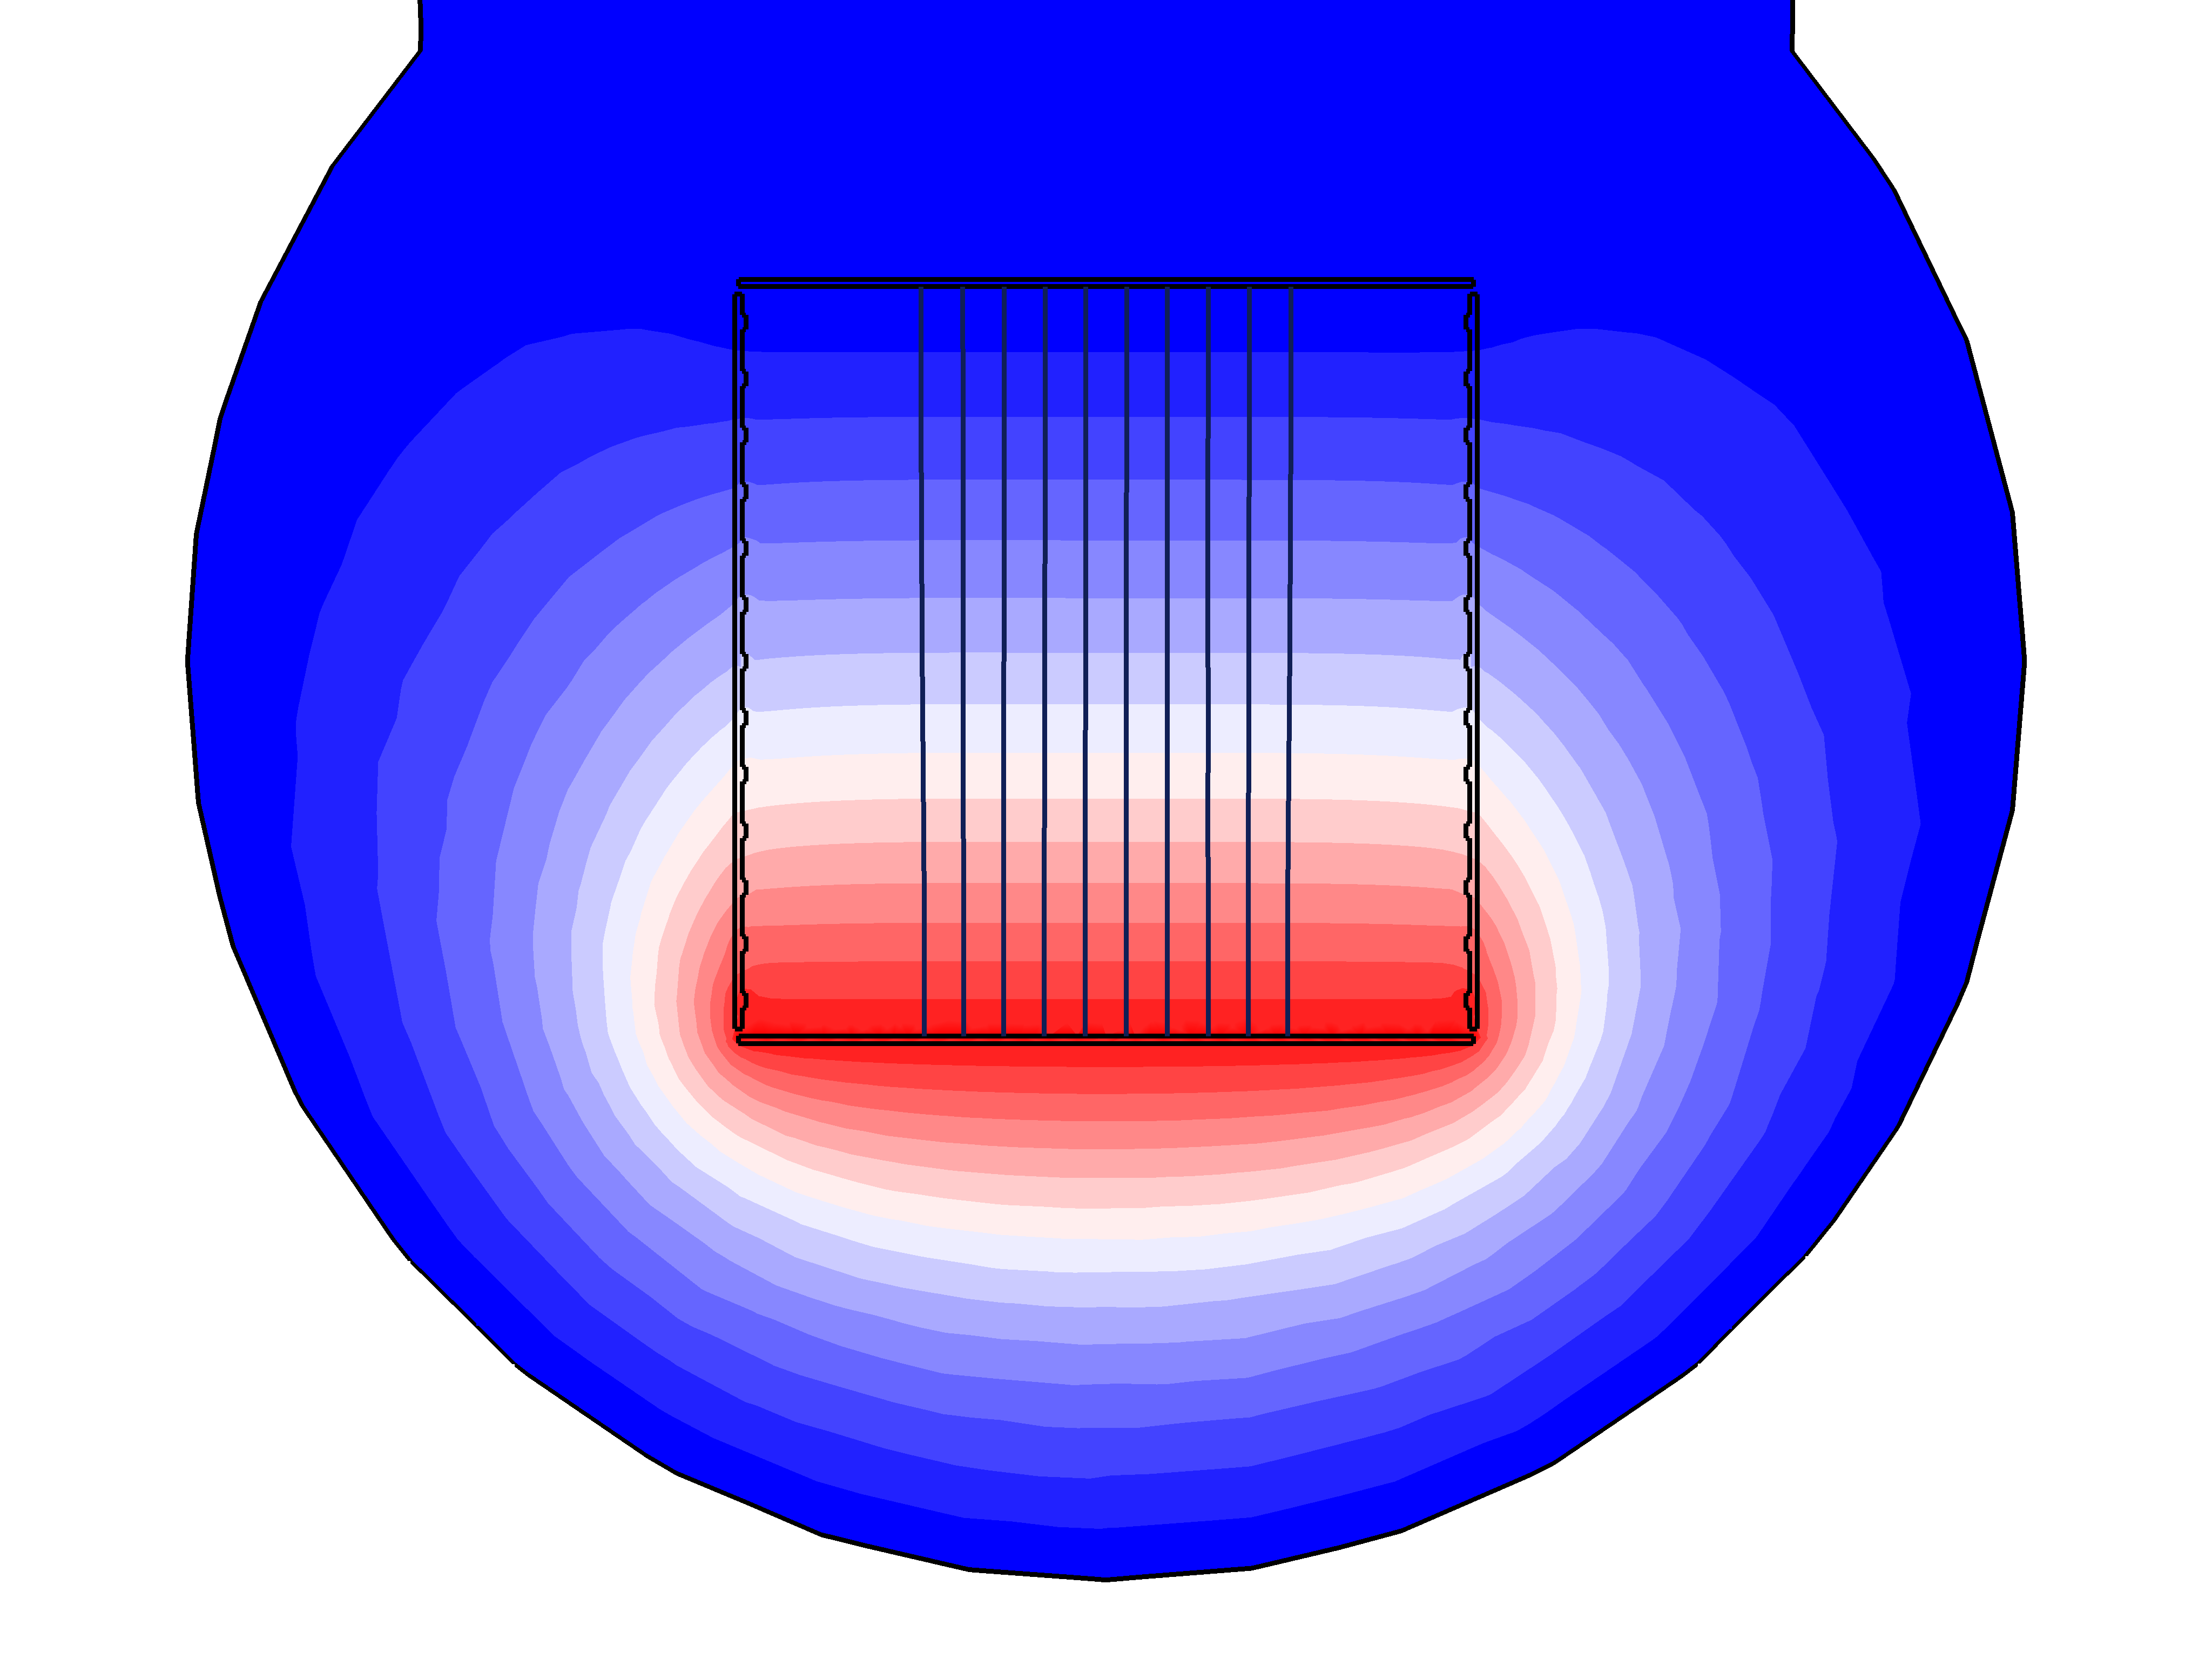
\includegraphics[width=0.9\textwidth]{03_SIM/fig/fig000_Lines_Corr}}
      \end{center}
    \end{column}
  \end{columns}
\end{frame}

\begin{frame}[t]
  \frametitle{Field uniformity}
  \begin{columns}[T]
    \begin{column}{0.45\textwidth}
      3 main leverages
      \begin{block}{IPM position and geometry}
        Vacuum geometry is frozen $\rightarrow$ limited solution
      \end{block}
      \begin{block}{Disks}
        Reduce the cross-interaction.

        Each IPM becomes a unique system.
      \end{block}
      \begin{block}{Field correctors}
        The field is constrained inside the cage.

        Shield IPM from external devices (HV wires).
      \end{block}
    \end{column}
    \begin{column}{0.45\textwidth}
      E. field computed using FEM COMSOL and an in-house C++ particle tracking is used.
      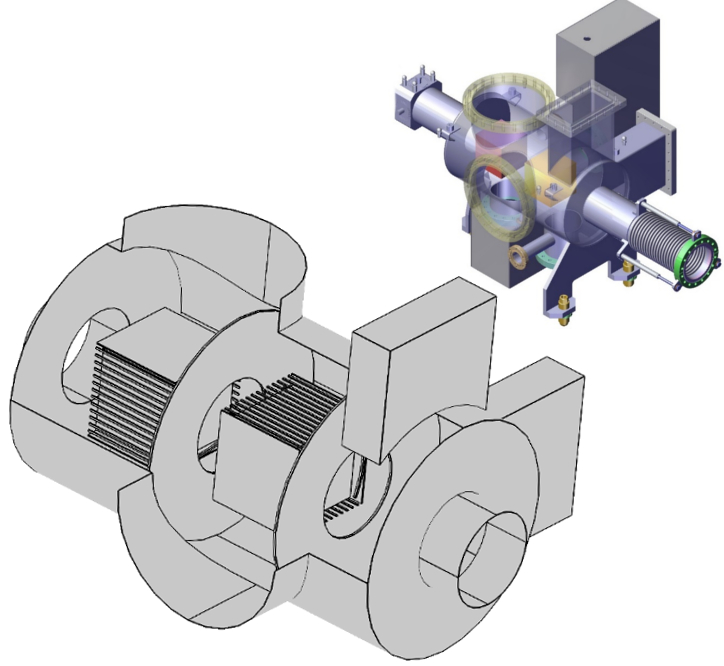
\includegraphics[width=1\textwidth]{03_SIM/fig/fig003_COMSOL_LWU2}

    \end{column}
  \end{columns}
\end{frame}

\begin{frame}[t]
  \frametitle{Field uniformity}
  \begin{center}
    \only<1>{%
      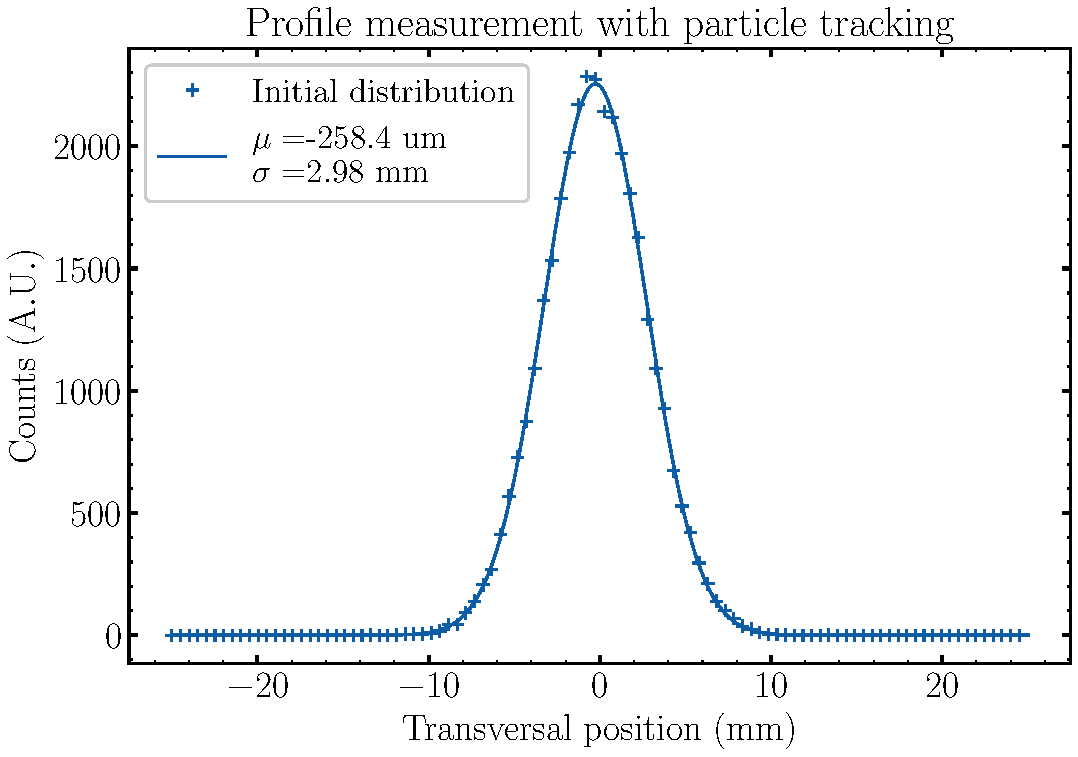
\includegraphics[width=0.7\textwidth]{03_SIM/fig/fig000_track_comsol_1}%
    }%
    \only<2>{%
      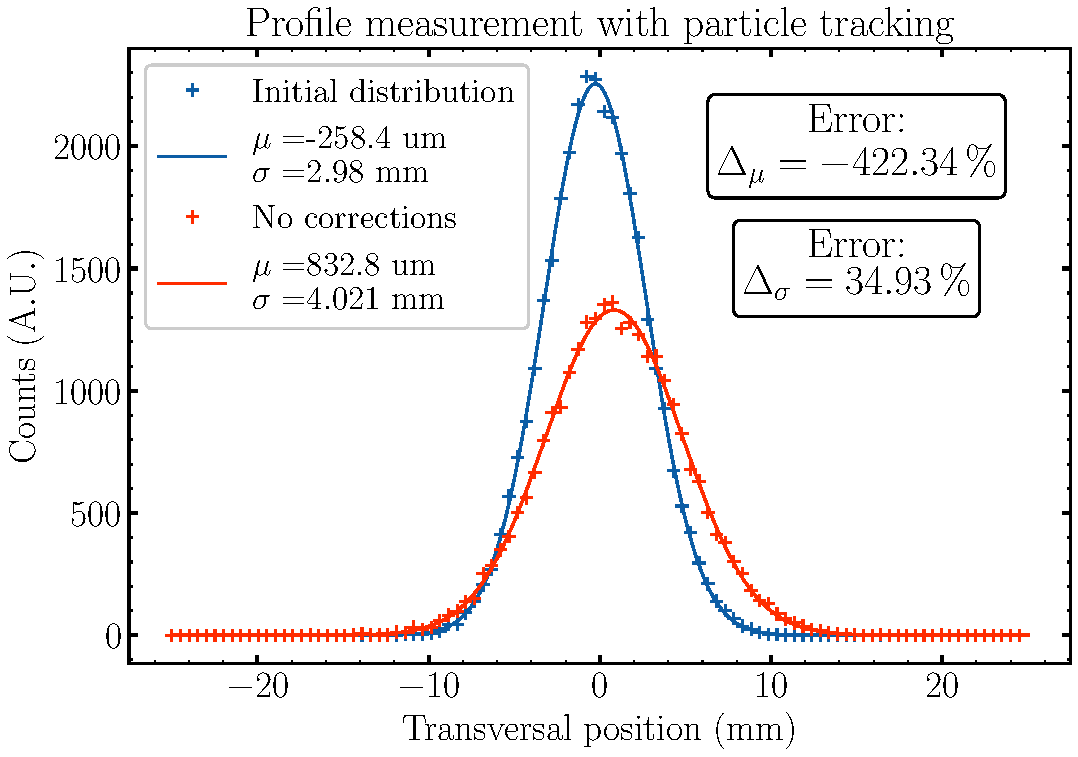
\includegraphics[width=0.7\textwidth]{03_SIM/fig/fig000_track_comsol_2}%
    }%
    \only<3>{%
      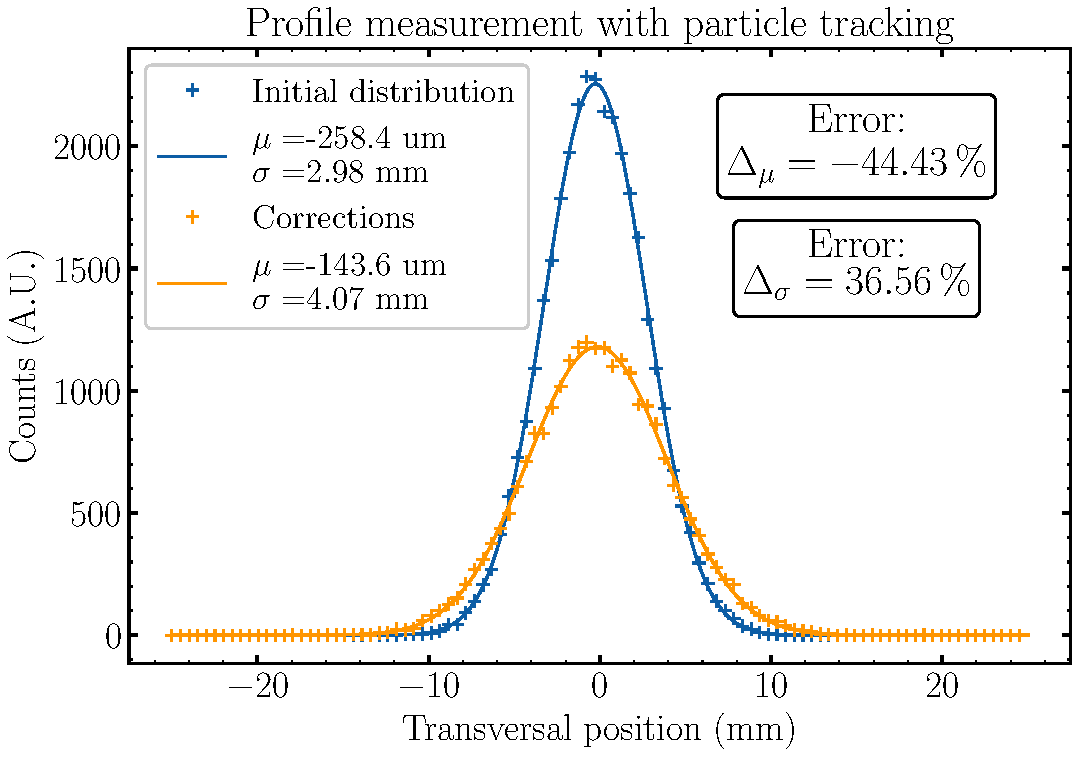
\includegraphics[width=0.7\textwidth]{03_SIM/fig/fig000_track_comsol_3}%
    }%
    \only<4->{%
      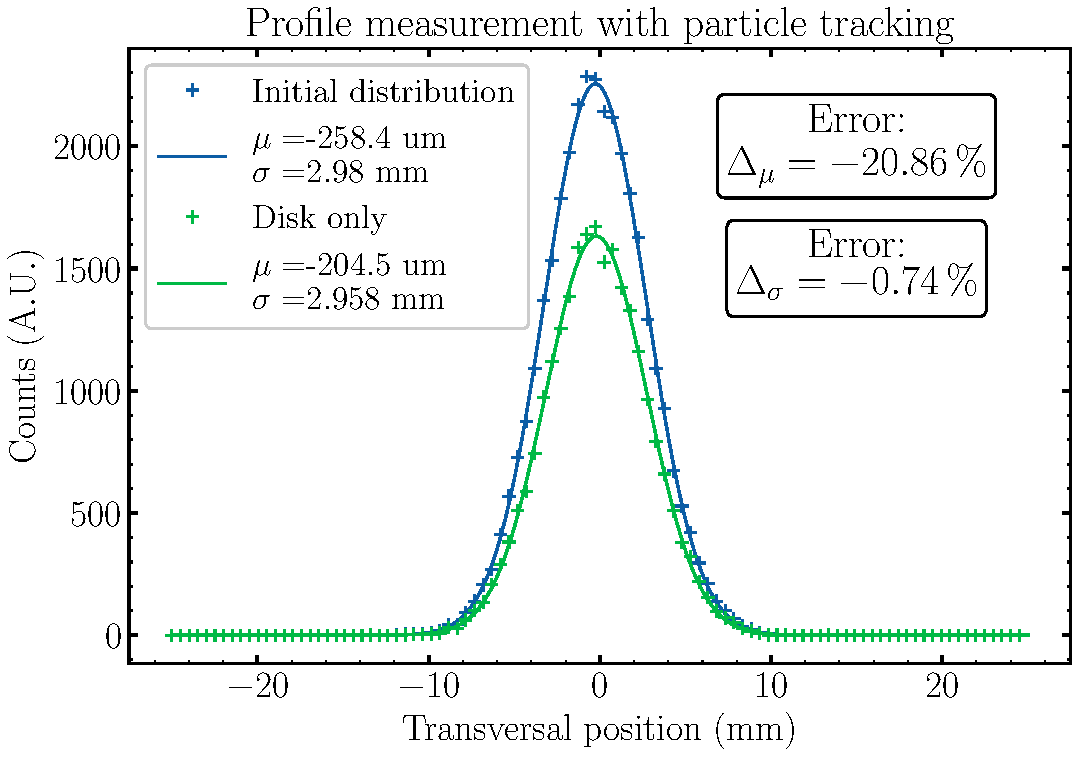
\includegraphics[width=0.7\textwidth]{03_SIM/fig/fig000_track_comsol_4}%
    }% 
  \end{center}
  \only<5>{%
    \begin{alertblock}{Conclusion}%
      Hardware corrections are mandatory since they reduce significantly the non uniformities.%
    \end{alertblock}%
  }%
\end{frame}

% \begin{frame}[t]
%   \frametitle{Field uniformity}
%   \begin{columns}
%     \begin{column}{0.5\textwidth}

%     \end{column}
%     \begin{column}{0.5\textwidth}

%     \end{column}
%   \end{columns}
% \end{frame}

% \begin{frame}[t]
%   \frametitle{Field uniformity}
%   \begin{itemize}
%     \item IPM geometry itself, side effects
%     \item The vacuum vessel that encloses the IPM
%     \item IPM polarization
%     \item Others devices in vacuum
%   \end{itemize}
%   Electrostatic field can be computed on 3D domain using FEM $\rightarrow$ COMSOL in our case
% \end{frame}

\subsection{Space charge}
\begin{frame}[t]
  \frametitle{Space charge}
  \begin{block}{Definition}
    The space charge refers to the effect of moving proton bunches on the profile measurement: moving bunches generate an important EM field that affects the drift of the electrons/ions.
  \end{block}
  An algorithm has been developed by C. Thomas (ESS) and F. Belloni (CEA):
  %\begin{columns}
  %  \begin{column}{0.45\textwidth}
  \begin{block}{Algorithm in brief}
    \begin{itemize}
      \item Compute electric field of gaussian bunches in the moving frame.
      \item Lorentz transformation in the IPM frame $\implies$ EM field
      \item Particles tracking
    \end{itemize}
  \end{block}
  %  \end{column}
  %  \begin{column}{0.45\textwidth}
  %  \end{column}
  % \end{columns}
  \begin{block}{Information}
    The space charge can be compensated:
    \begin{itemize}
      \item By adding a magnetic field about hundred $mT$ $\rightarrow$ impossible in our case
      \item By increasing the E field but limited by power supplies, sparks ...
    \end{itemize}
  \end{block}
\end{frame}

\begin{frame}[t]
  \frametitle{Space charge}
  \begin{block}{Generalities}
    \begin{itemize}
      \item The space charge effect is more important at "low" beam energy.
      \item The space charge effect increases with beam current.
    \end{itemize}
  \end{block}
  Example with worst ESS case: $90\,\mathrm{MeV}$ $62.5\,\mathrm{mA}$
  \begin{columns}[T]
    \begin{column}{0.45\textwidth}
      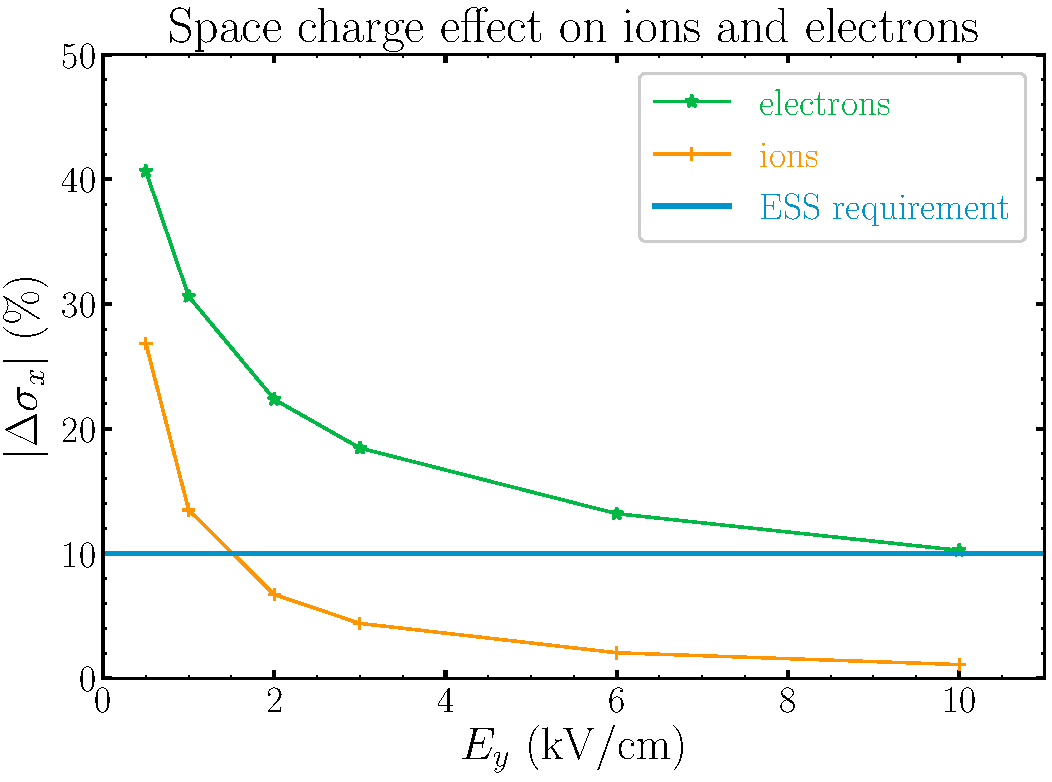
\includegraphics[width=0.95\textwidth]{03_SIM/fig/fig000_SC_ions_electrons}
    \end{column}
    \begin{column}{0.45\textwidth}
      \begin{overlayarea}{\textwidth}{2cm}
        \only<1>{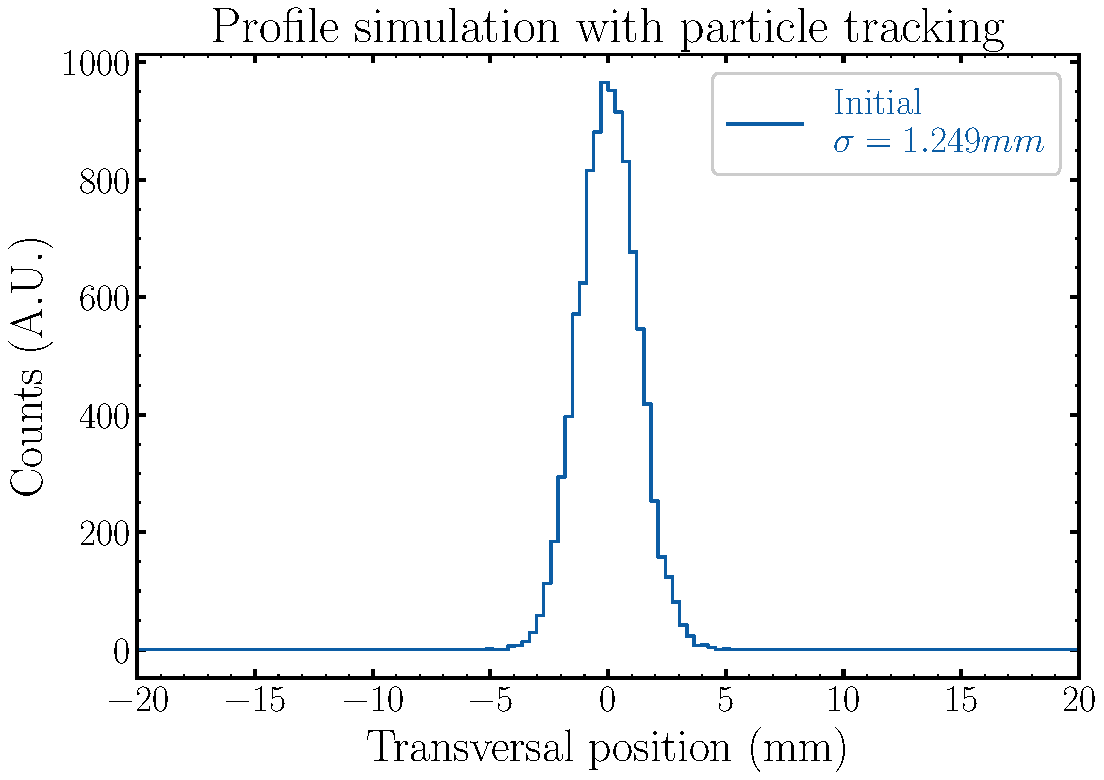
\includegraphics[width=\textwidth]{03_SIM/fig/fig000_SC}}
        \only<2>{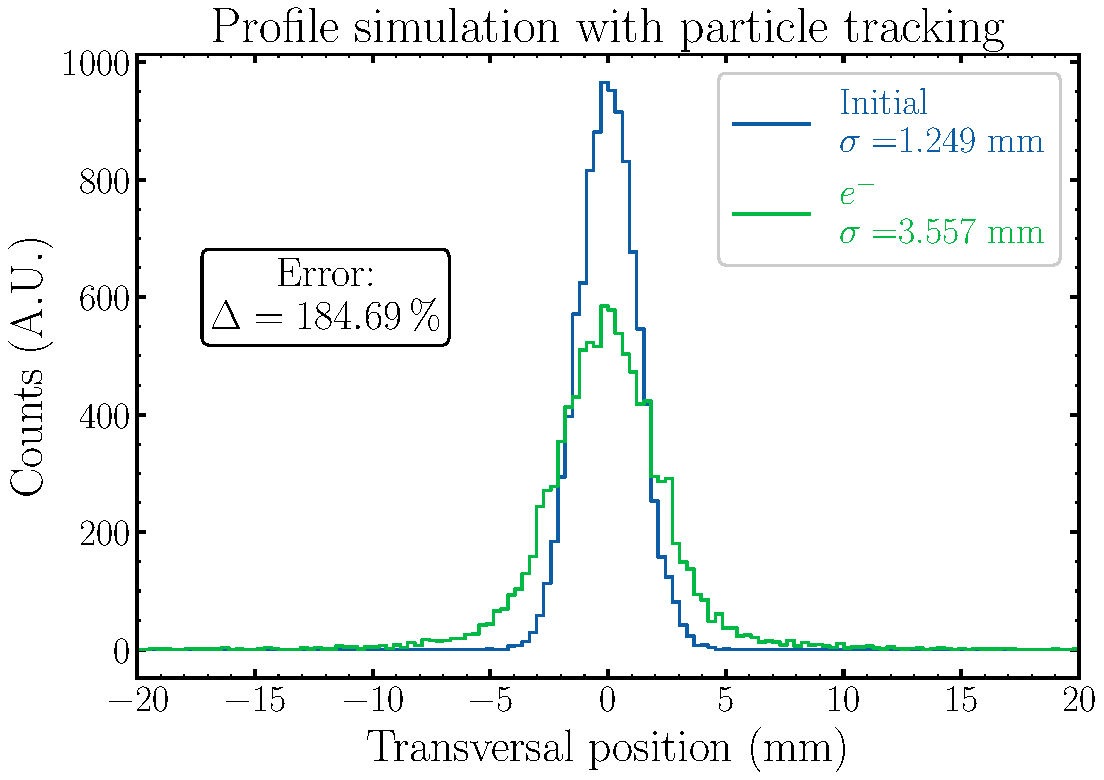
\includegraphics[width=\textwidth]{03_SIM/fig/fig000_SC_electron}}
        \only<3>{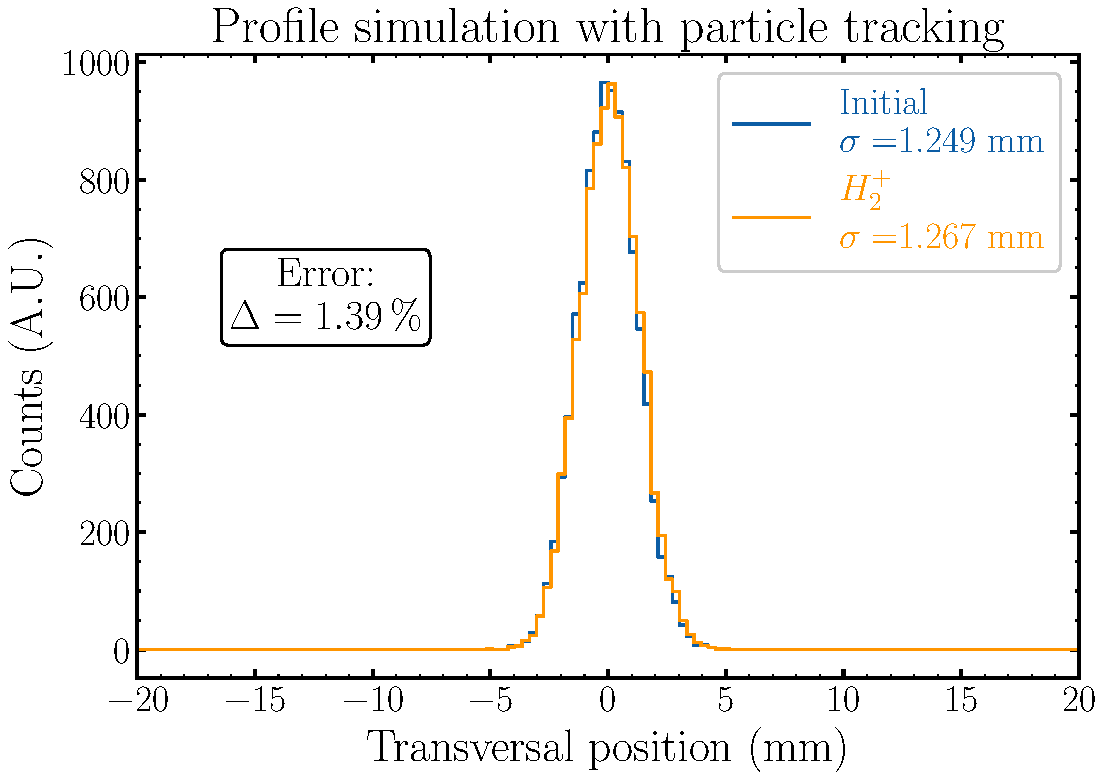
\includegraphics[width=\textwidth]{03_SIM/fig/fig000_SC_ions}}
      \end{overlayarea}
    \end{column}
  \end{columns}
  \begin{alertblock}{Conclusion}
    The measurement with electrons does not meet the ESS requirements.
    The profile measurement must be performed with ions.
  \end{alertblock}
\end{frame}

\subsection{Readout}
\begin{frame}[t]
  \frametitle{Strips (multi anodes)}
  \begin{block}{How does it work?}
    A moving particle induces a current on the anodes. The anodes are read by charge integrator or transimpedance.
  \end{block}
  \begin{columns}[T]
    \begin{column}{0.45\textwidth}
      \begin{block}{Pros}
        \begin{itemize}
          \item Simple to implement
          \item Robust
        \end{itemize}
      \end{block}
    \end{column}
    \begin{column}{0.45\textwidth}
      \begin{block}{Cons}
        \begin{itemize}
          \item No amplification
          \item Sensitive electronics (high gain, high BW)
        \end{itemize}
      \end{block}
    \end{column}
  \end{columns}

  \begin{columns}[]
    \begin{column}{0.45\textwidth}
      \begin{block}{Prototype}
        \begin{itemize}
          \item 32 strips linearly spaced with $800\,\mathrm{\mu m}$ width.
          \item COTS 32 channel charge integrator, CARAMEL (LPC-Caen/CNRS).
        \end{itemize}
      \end{block}
    \end{column}
    \begin{column}{0.45\textwidth}
      \centering
      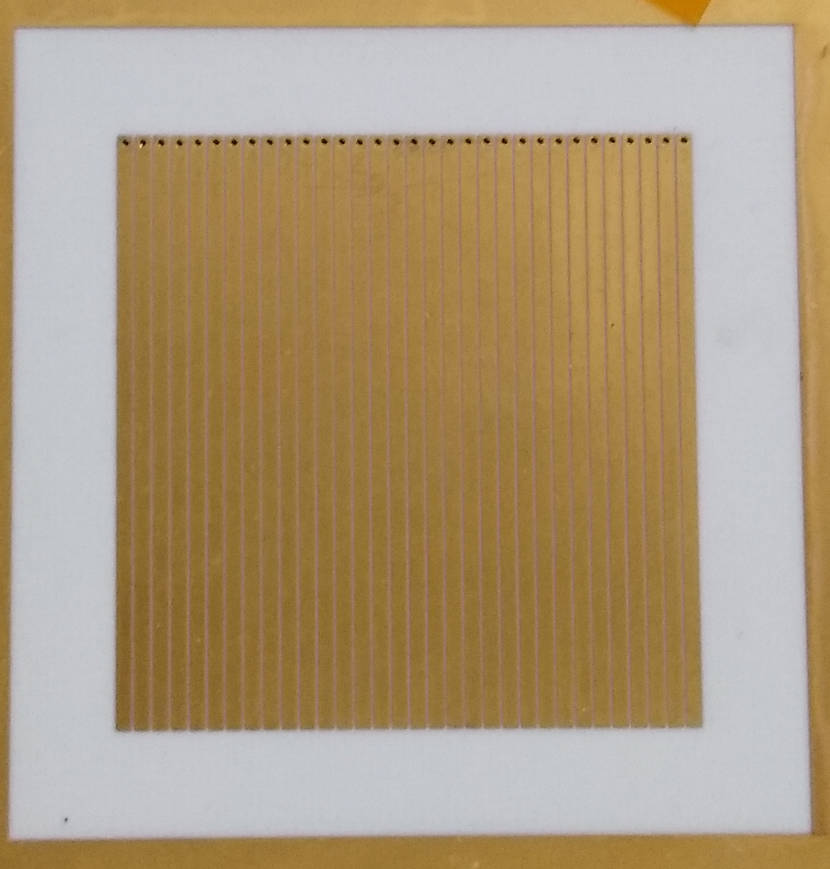
\includegraphics[width=0.5\textwidth]{03_SIM/fig/fig000_strips2}
    \end{column}
  \end{columns}
\end{frame}

\begin{frame}[t]
  \frametitle{Micro Channel Plate}
  \begin{block}{How does it work?}
    Incident particles are amplified into electrons in a channel ($\approx 15\,\mathrm{\mu m}$)
  \end{block}

  \begin{columns}[T]
    \begin{column}{0.45\textwidth}
      \begin{center}
        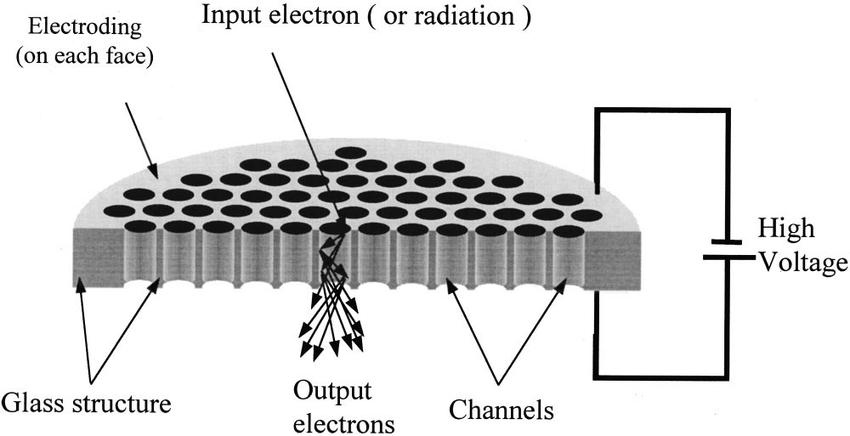
\includegraphics[width=1\textwidth]{03_SIM/fig/fig00_MCP_outline}
      \end{center}
    \end{column}
    \begin{column}{0.45\textwidth}
      \begin{center}
        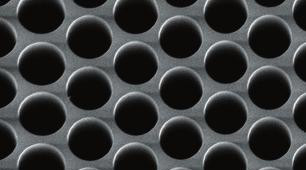
\includegraphics[width=1\textwidth]{03_SIM/fig/fig000_MCP_outline_b2}
      \end{center}
    \end{column}
  \end{columns}

  \begin{columns}
    \begin{column}{0.45\textwidth}
      \begin{block}{Pros}
        \begin{itemize}
          \item Huge amplification
          \item Can be stacked
          \item High ion sensitivity
        \end{itemize}
      \end{block}
    \end{column}
    \begin{column}{0.45\textwidth}
      \begin{block}{Cons}
        \begin{itemize}
          \item Ageing
          \item Saturation
          \item Fragile devices
        \end{itemize}
      \end{block}
    \end{column}
  \end{columns}
\end{frame}

\begin{frame}[t]
  \frametitle{Micro Channel Plate}
  \begin{block}{Readout and electronics}
    MCP is just an amplifier, a readout must be coupled:
    \begin{columns}[T]
      \begin{column}{0.45\textwidth}
        \begin{itemize}
          \item Multiple anodes
        \end{itemize}
      \end{column}
      \begin{column}{0.45\textwidth}
        \begin{itemize}
          \item Phosphorus screen
        \end{itemize}
      \end{column}
    \end{columns}
  \end{block}
  \begin{block}{Prototype}
    Single stage MCP from Hamamatsu and Photonis with P46 (fast) and P43 (slow) screen. COTS camera and lens were used to record light from screen
  \end{block}

  \begin{columns}[T]
    \begin{column}{0.25\textwidth}
      \centering
      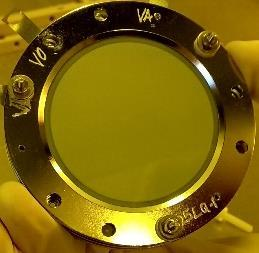
\includegraphics[width=0.7\textwidth]{03_SIM/fig/fig000_MCP_photo}
      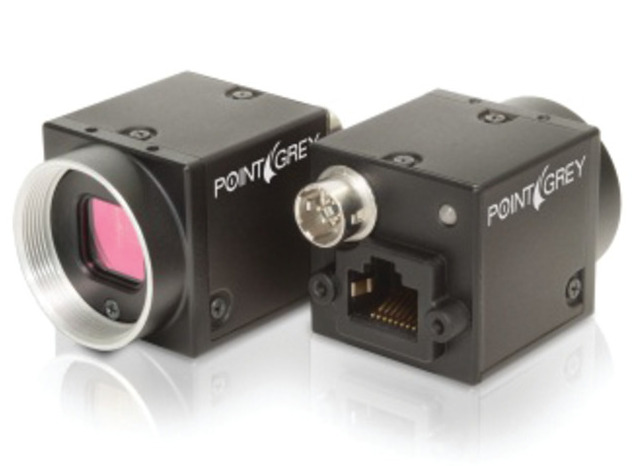
\includegraphics[width=1\textwidth]{03_SIM/fig/fig000_MCP_camera}
    \end{column}
    \begin{column}{0.65\textwidth}
      \begin{tabularx}{\linewidth}{XX}
        \toprule
        Property        & Value                                            \\
        \midrule
        Resolution      & $1936\,\mathrm{(H)}\,\times\,1216\,\mathrm{(V)}$ \\
        Pixel size      & $5.86\,\mathrm{\mu m}$                           \\
        Sensor diag.    & $13.4\,\mathrm{mm}$                              \\
        Well capacity   & $32000\,\mathrm{e^{-}}$                          \\
        Dynamic range   & $70\,\mathrm{dB}$                                \\
        QE at 525 nm    & $70\,\mathrm{\%}$                                \\
        Electrons noise & $6.8\,\mathrm{e^{-}}$                            \\
        \bottomrule
      \end{tabularx}
    \end{column}
  \end{columns}
\end{frame}

\begin{frame}[t]
  \frametitle{Hybrid Pixel Detector}
  The use of silicon detector is new for IPM and was initiate by CERN teams.
  \begin{block}{How does it work?}
    Incident particles generate $e^{-}$/ion pairs in silicon sensor that collected by a readout circuit.
  \end{block}
  \begin{columns}[T]
    \begin{column}{0.45\textwidth}
      \centering
      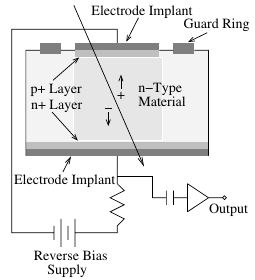
\includegraphics[width=0.5\textwidth]{03_SIM/fig/fig000_Si_detector}
    \end{column}
    \begin{column}{0.45\textwidth}
      \centering
      A TimePix3 chip: $1.4\times1.4\,\mathrm{cm}$
      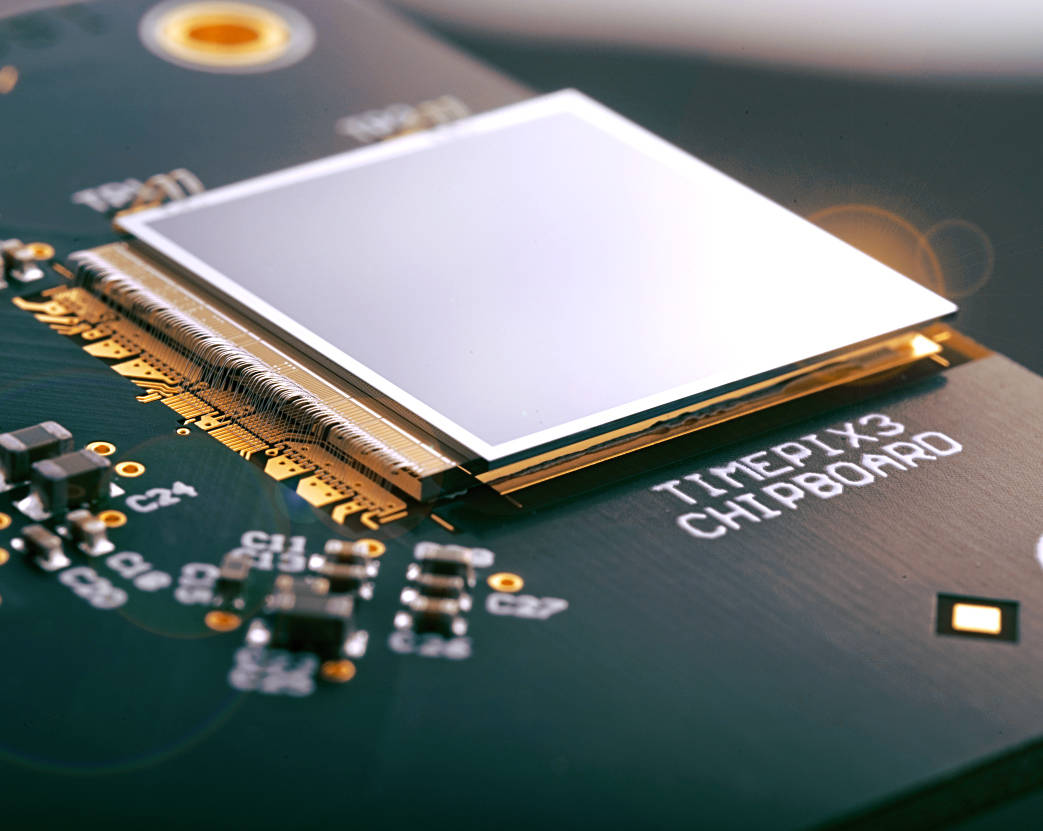
\includegraphics[width=0.6\textwidth]{03_SIM/fig/fig000_TimePix3}
    \end{column}
  \end{columns}

  \begin{columns}[T]
    \begin{column}{0.45\textwidth}
      \begin{block}{Pros}
        \begin{itemize}
          \item Amplification
          \item Fast timing (Time of Arrival (ToA), $1.56\,\mathrm{ns}$)
        \end{itemize}
      \end{block}
    \end{column}
    \begin{column}{0.45\textwidth}
      \begin{block}{Cons}
        \begin{itemize}
          \item Implementation (electronics design, cooling)
          \item Use of ion (next slide)
        \end{itemize}
      \end{block}
    \end{column}
  \end{columns}
\end{frame}

\begin{frame}[t]
  \frametitle{Hybrid Pixel Detector}
  \begin{columns}[T]
    \begin{column}{0.45\textwidth}
      \begin{block}{Prototype}
        The CERN team kindly provided us a FitPix kit (TimePix1 + Si sensor).
      \end{block}
    \end{column}
    \begin{column}{0.45\textwidth}
      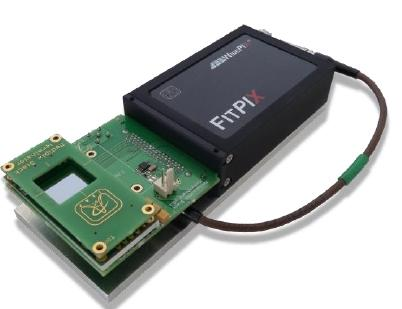
\includegraphics[width=0.8\textwidth]{03_SIM/fig/fig000_FitPix}
    \end{column}
  \end{columns}
  \vskip 0.5cm
  \begin{columns}[T]
    \begin{column}{0.45\textwidth}
      \begin{alertblock}{The use of ions}
        \begin{itemize}
          \item Multiple ion species $\implies$ impossible to solve the ToA.
          \item Low penetration depth, may be not detected.
          \item High damages in silicon.
        \end{itemize}
      \end{alertblock}
    \end{column}
    \begin{column}{0.45\textwidth}
      \centering
      Geant4 and SRIM simulations
      \only<1>{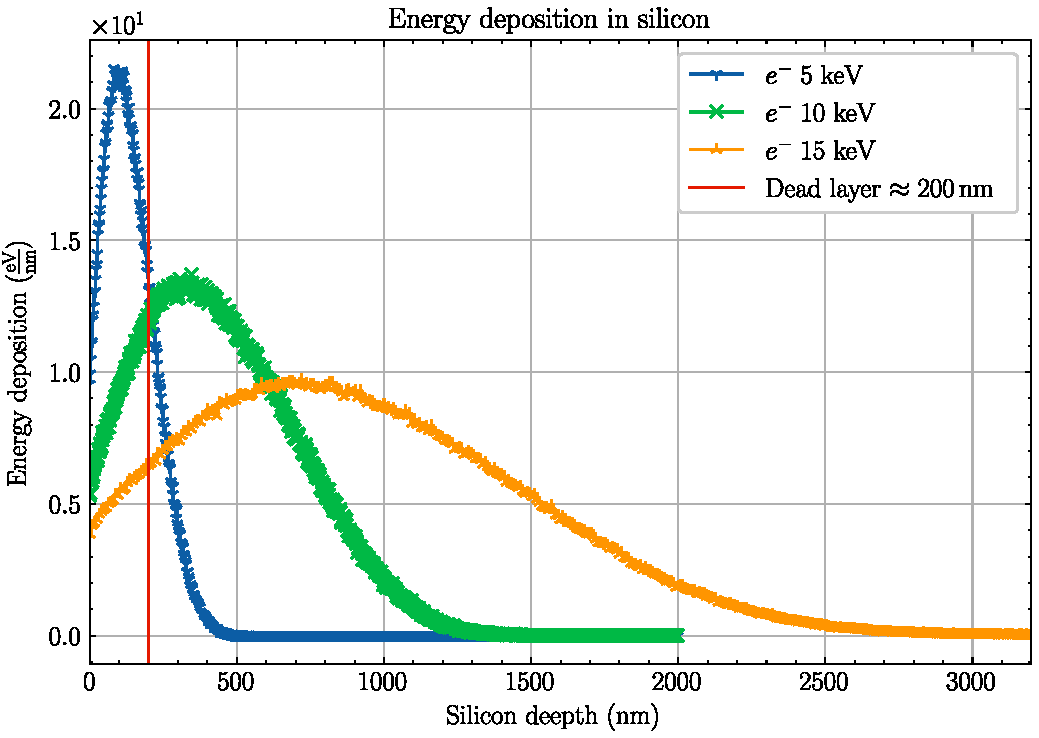
\includegraphics[width=\textwidth]{03_SIM/fig/fig011_electron_si_deposit}}
      \only<2>{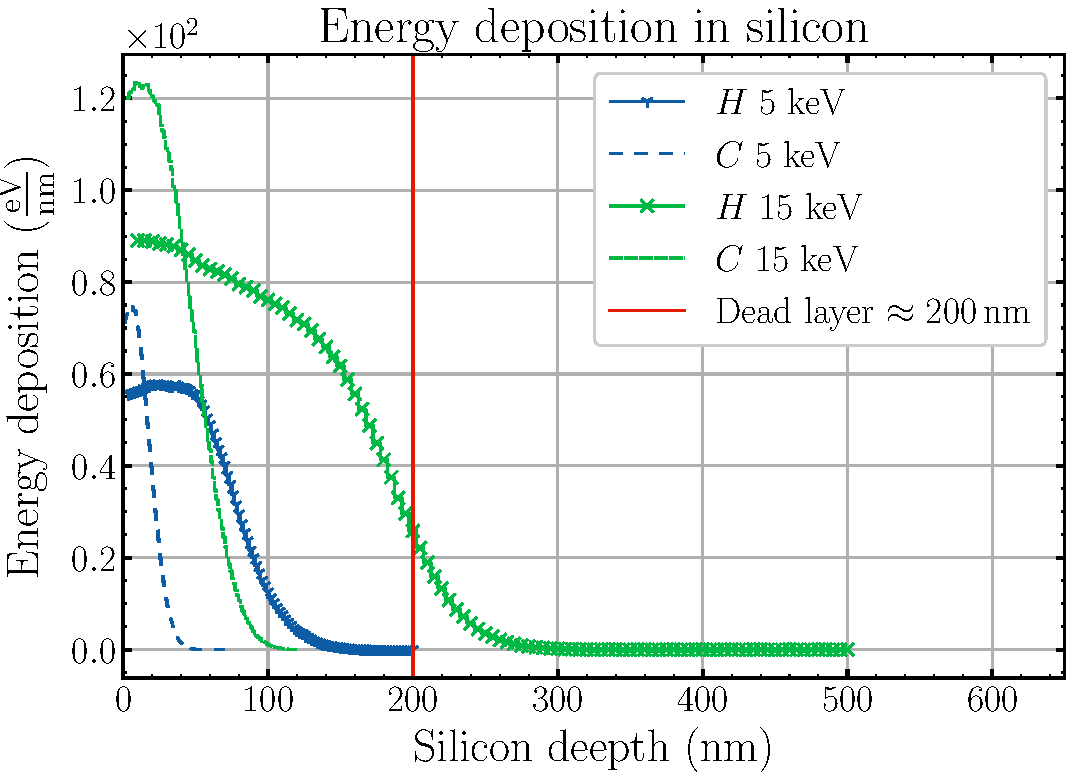
\includegraphics[width=\textwidth]{03_SIM/fig/fig011_ion_si_deposit}}
    \end{column}
  \end{columns}

\end{frame}

\begin{frame}[t]
  \frametitle{Summary}
  \begin{block}{3 types of IPM are forseen for ESS}
    Which one is the best for the ESS cold linac?
  \end{block}
  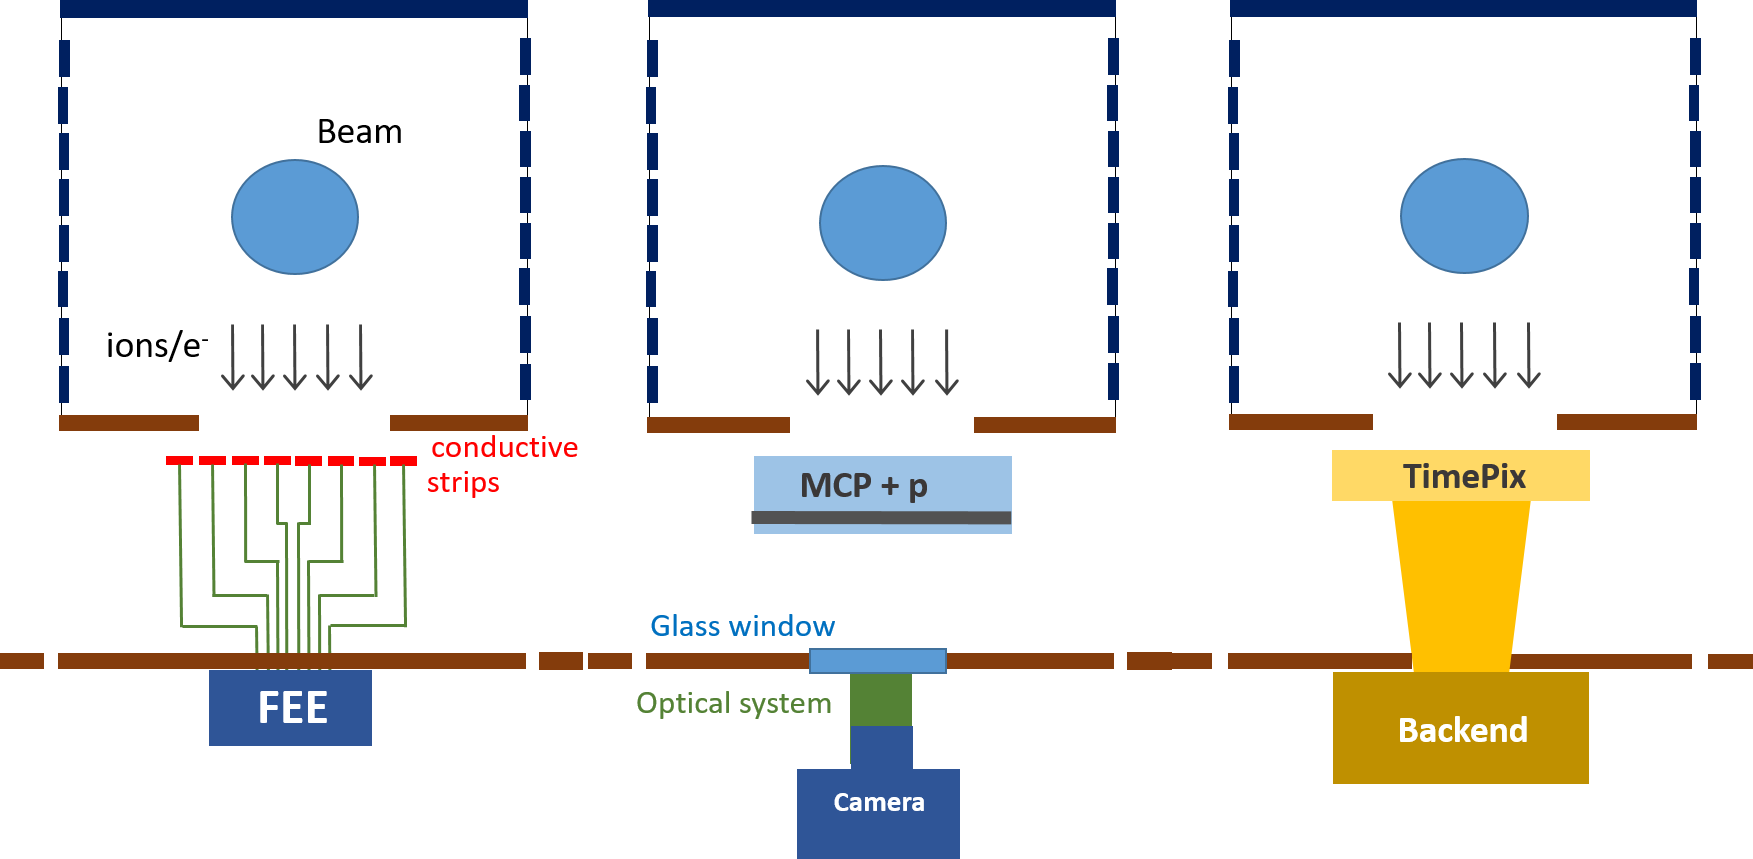
\includegraphics[width=1\textwidth]{03_SIM/fig/fig000_recap}
\end{frame}